\chapter{Processo de Engenharia de Requisitos}

  Neste tópico será apresentado o processo de Engenharia de Requisitos que será executado no projeto, descrevendo quais os papeis,
  e sua respectiva modelagem criada na ferramenta draw.io, que é uma ferramenta online de desenhos UML e de modelagem.

  Logo abaixo será especificado como tratam sobre o modelo do processo de Engenharia de Requisitos, apelidado de \textbf{Big Picture}
  do projeto, os papéis desempenhados e as atividades e artefatos envolvidos no processo.

\section{Modelo de Processo de Engenharia de Requisitos}

  \begin{figure}[!htb]
    \centering
    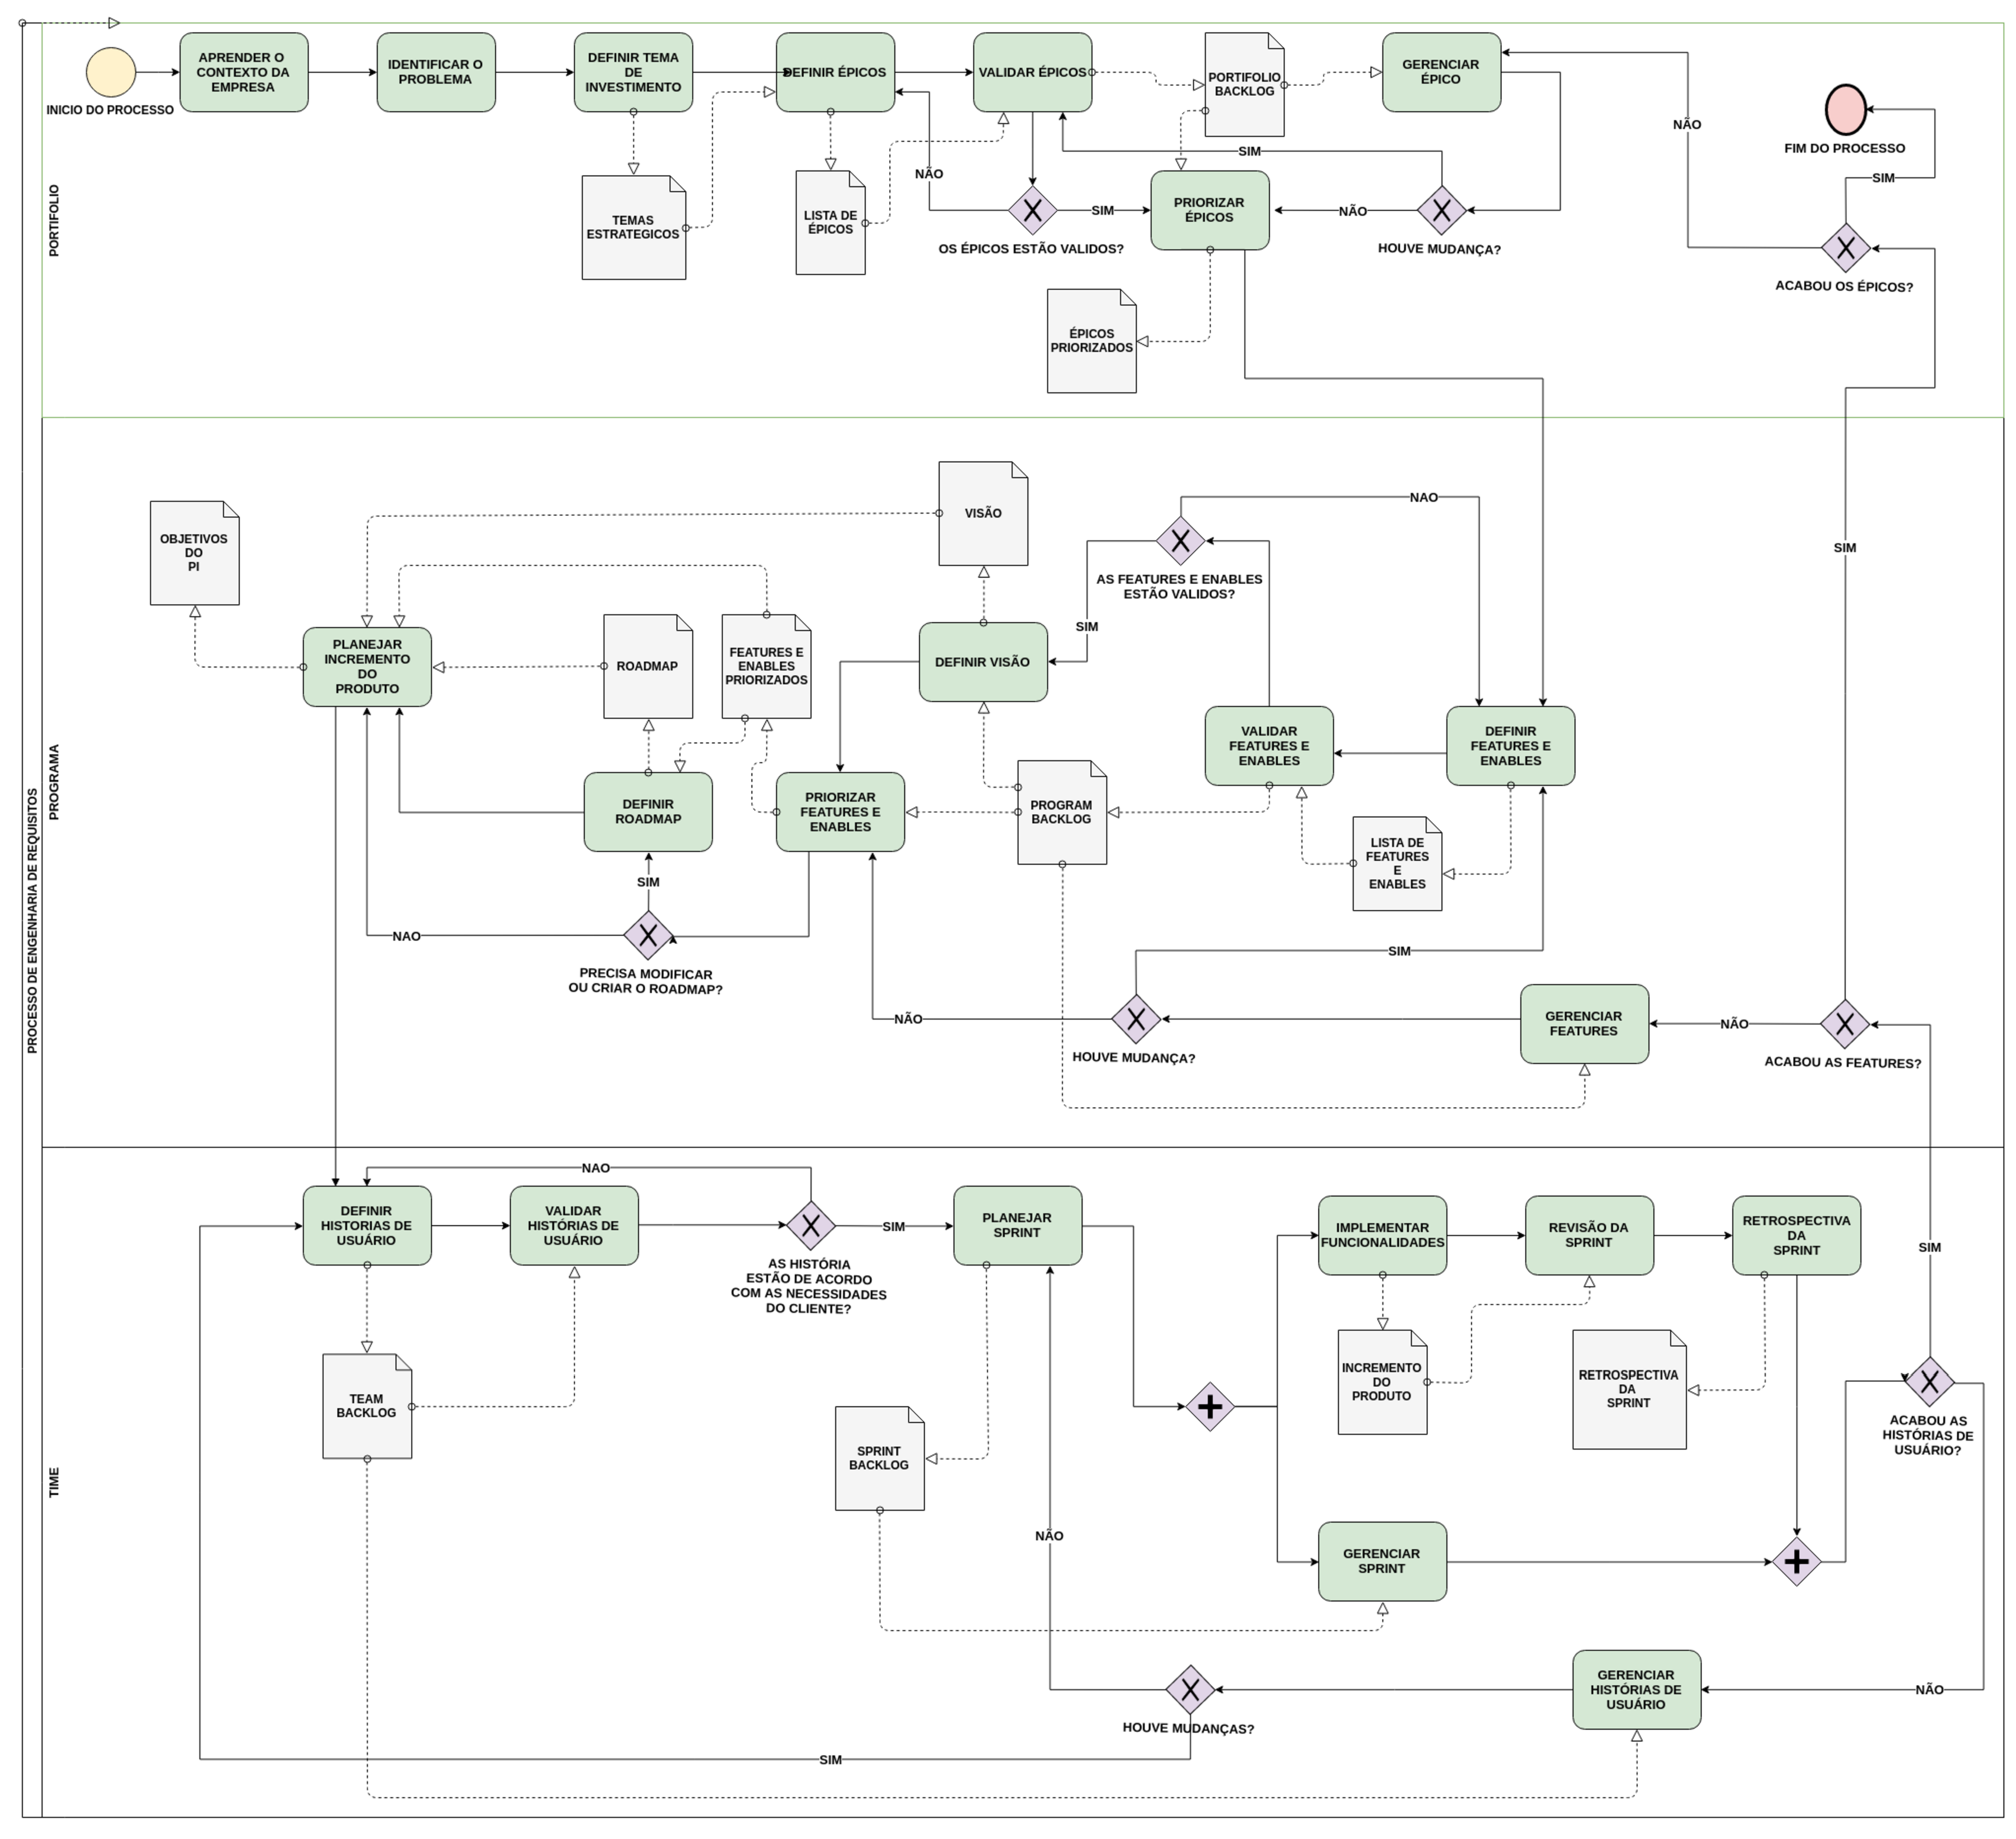
\includegraphics[width=15cm, keepaspectratio=true]{figuras/processo/processo.eps}
    \caption{Processo da Engenharia de Requisitos}
  \end{figure}

\section{Papéis}

\subsection{\textbf{Portfólio}}

  \begin{itemize}
    \item \textbf{Gerente de Portfólio de Programa}: Representa a pessoa que tem mais impacto nas decisões tantos estratégicas quanto
      financeiras dentro do framework, e entende os limites da estratégia de negócio da empresa, de tecnologia e de fundos. Uma de suas
      responsabilidades é de participar das sessões de escolha e comunicação dos temas de investimento e da definição e priorização do
      backlog de épicos.
    \item \textbf{Gerente de Épicos}: Representa o papel na qual toma-se a responsabilidade de gerenciar épicos individuais por todo o
      processo de portifolio kanban, desenvolvendo casos de negócios. Trabalha-se com os principais stakeholders na análise de valor
      agregado do épico. Quando o épico é aprovado, o gerente de épico trabalha com o time de desenvolvimento e o gerente de produto
      para estabelecer as atividades de desenvolvimento, para que as mesmas atinjam os benefícios de negócios do épico em especifico.
    \item \textbf{Arquiteto da empresa}: Representa a pessoa que sempre visa manter uma visão geral das tecnologias, soluções da
      empresa e iniciativas de desenvolvimento. Uma de suas atividades é entender e comunicar os temas de investimento e outras chaves
      de negócios para os arquitetos de sistema e stakeholders não técnicos, e também influenciar na decisão de uma modelagem comum e
      em boas práticas de codificação.
  \end{itemize}

\subsection{\textbf{Programa}}

  \begin{itemize}
    \item \textbf{Gerente de Releases}: Representa a pessoa que planeja a release, e coordena a implementação de todas as capacidades e
      funcionalidades nas diversas iterações dentro de uma release. Um de seus papéis é comunicar o status da release para stakeholders
      externos a empresa, e também de prover uma autorização final da release.
    \item \textbf{Gerente de Produto}: Junto do Gerente de Soluções, eles formam as principais autoridades de conteúdo. Eles criam a
      visão do programa, trabalham com os clientes e também com os Product Owners para entenderem e comunicarem as necessidades,
      participam na validação de soluções propostas, define os requisitos, gerencia e prioriza o fluxo de trabalho e também define
      releases e Program Increments.
  \end{itemize}

\subsection{\textbf{Time}}

  \begin{itemize}
    \item \textbf{Product Owner (P.O)}: Representa a pessoa que tem como responsabilidade a definição das histórias de usuário e de
      priorizar o backlog de time. O P.O desempenha um papel importantíssimo no quesito qualidade, pois é o único do time que tem a
      responsabilidade de aceitar as histórias como finalizadas. É bastante envolvido na construção do backlog do programa e na
      preparação e refinamento do planejamento do PI
    \item \textbf{Scrum Master}: Representa a pessoa que está sempre monitorando a equipe com o intuito de fazer com que todos sigam
      a metodologia, ou seja, o Scrum Master monitora os integrantes para que todos cumpram e sigam os princípios da metodologia.
      Uma das responsabilidades do Scrum Master é manter a equipe focada nos objetivos certos, assegurando um fluxo de produtividade
      o mais alto possível. Também tem como responsabilidade facilitar os encontros do time, tanto no planejamento quanto na
      retrospectiva e revisão da sprint.
    \item \textbf{Desenvolvedores}: Representa as pessoas que vão de fato construir o sistema, produzindo o código fonte e os testes
      da aplicação. Participa de todas as atividades do processo no nível de time.
    \item \textbf{Equipe}: Representa a junção dos três citados acima.
  \end{itemize}

